\documentclass[12pt, a4paper, oneside]{article}
\usepackage{arial}
\renewcommand{\familydefault}{\sfdefault}
\usepackage[T1]{fontenc}
\usepackage[polish]{babel}
\usepackage[utf8]{inputenc}
\usepackage{lmodern}
\usepackage[left=2cm,right=2cm,top=2cm,bottom=2cm]{geometry}
\selectlanguage{polish}
\usepackage{graphicx}
\usepackage{longtable}

\begin{document}
\section{Wykorzystane wzory}
Niepewność zmierzonej długości linii
\begin{equation}
u(L)=\frac{\Delta_{siatki}}{\sqrt{3}}
\end{equation}
Powiększenie interferometru
\begin{equation}
k=\frac{L_1}{L_0}
\end{equation}
Niepewność wyznaczonego powiększenia interferometru
\begin{equation}
u_C(k)=\sqrt{(\frac{\partial k}{\partial L_0})^2\cdot u^2(L_0)+(\frac{\partial k}{\partial L_1})^2\cdot u^2(L_1)}=\sqrt{\frac{L_1^2}{L_0^4}\cdot u^2(L_0)+\frac{1}{L_0^2}\cdot u^2(L_1)}
\end{equation}
\section{Przykładowe obliczenia}
Niepewność zmierzonej długości linii
\begin{center}
$u(L)=\frac{0.1}{1.73}=0.058~[cm]$
\end{center}
Powiększenie interferometru
\begin{center}
$k=\frac{1.2}{1}=1.200$
\end{center}
Niepewność wyznaczonego powiększenia interferometru
\begin{center}
$u_C(k)=\sqrt{\frac{(1.2)^2}{1^4}\cdot(0.58)^2+\frac{1}{1^2}\cdot(0.58)^2}=0.091$
\end{center}
\clearpage
\section{Wyniki pomiarów i opracowanie}
\begin{figure}[h]
\centering
\caption{Odrysowana linia odniesienia pozwalająca określić powiększenie interferometru}
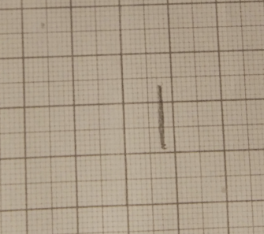
\includegraphics[scale=1]{pics/f1.png}
\end{figure}
\begin{figure}[h]
\centering
\caption{Prążki interferencyjne - próbka numer 1}
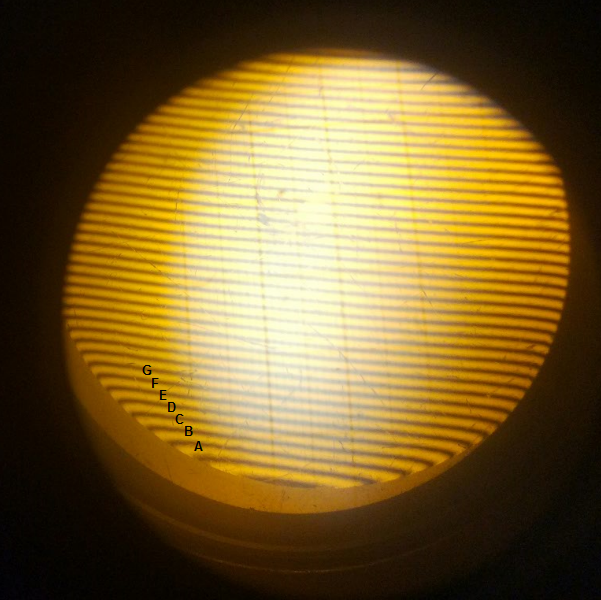
\includegraphics[scale=.55]{pics/f2.png}
\end{figure}
\clearpage
\begin{figure}[h]
\centering
\caption{Prążki interferencyjne - próbka numer 2}
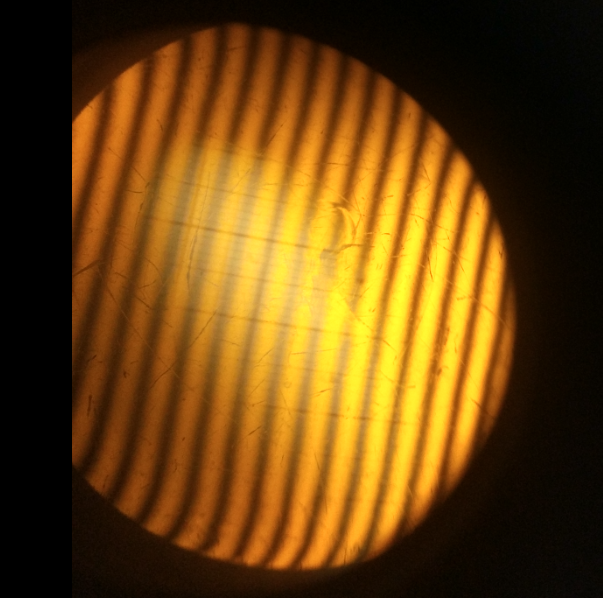
\includegraphics[scale=.4129]{pics/f3.png}
\end{figure}
\begin{figure}[h]
\centering
\caption{Prążki interferencyjne - próbka numer 3}
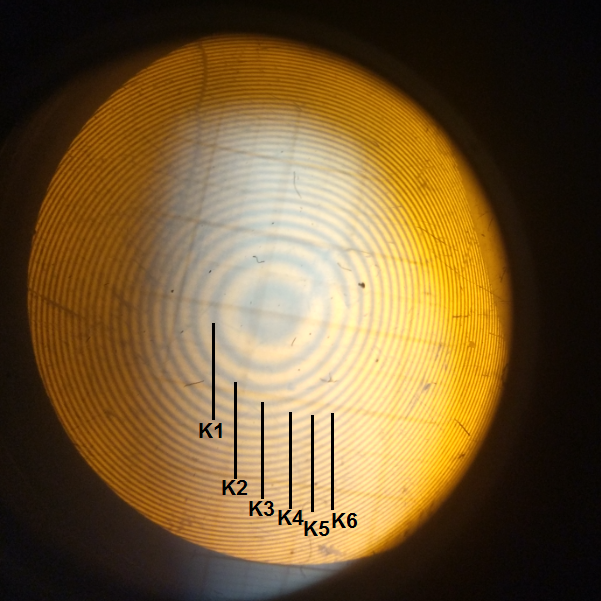
\includegraphics[scale=.55]{pics/f4.png}
\end{figure}
\clearpage
\begin{figure}[h]
\centering
\caption{Prążki interferencyjne - próbka numer 4}
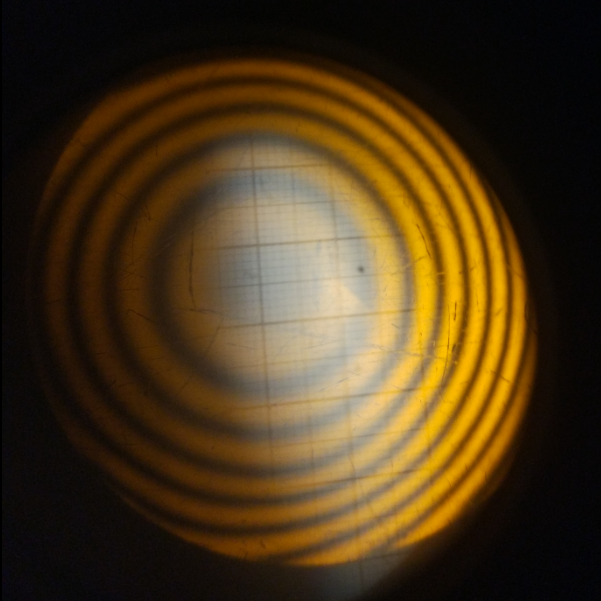
\includegraphics[scale=.4129]{pics/f5.png}
\end{figure}
\begin{figure}[h]
\centering
\caption{Prążki interferencyjne - próbka numer 5}
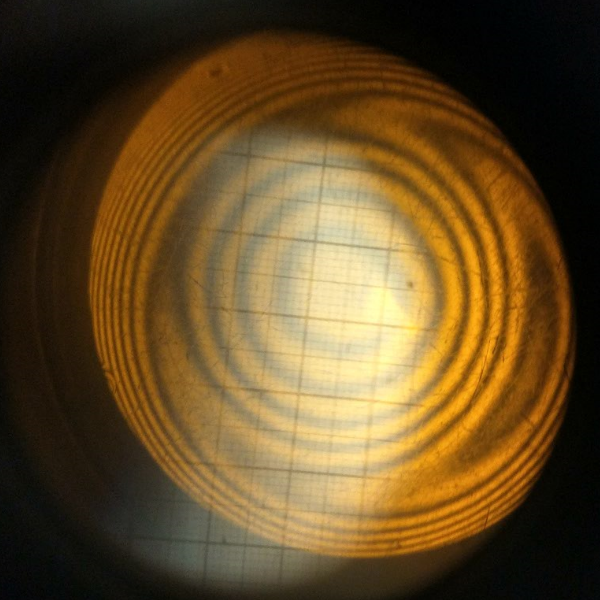
\includegraphics[scale=.4129]{pics/f6.png}
\end{figure}
\clearpage
\begin{figure}[h]
\centering
\caption{Prążki interferencyjne - próbka numer 6}
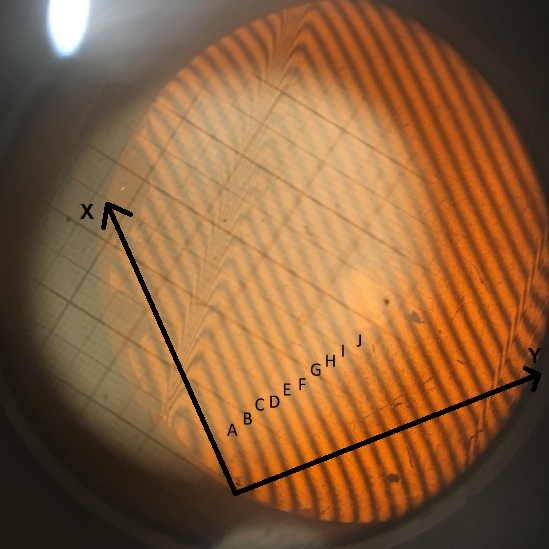
\includegraphics[scale=.4129]{pics/f7.png}
\end{figure}
\clearpage
\section{Wnioski}
\begin{itemize}
\item Powiększenie optyczne przyrządu wynosi k = 1.2 $\pm$ 0.091.
\end{itemize}
\end{document}